\documentclass[a4paper,12pt,twoside,openright,titlepage]{book}

%Additional packages
\usepackage[ascii]{inputenc}
\usepackage[T1]{fontenc}
\usepackage[dutch,english]{babel}
\usepackage{syntonly}
\usepackage[official]{eurosym}
%\usepackage[graphicx]
\usepackage{graphicx}
\graphicspath{ {./images/} }
\usepackage{float}
\usepackage{xurl}
\usepackage{hyperref}
\hypersetup{colorlinks=true, linkcolor=blue, citecolor=blue, filecolor=blue, urlcolor=blue, pdftitle=, pdfauthor=, pdfsubject=, pdfkeywords=}
\usepackage{tabularx}
\usepackage{scrextend}
\addtokomafont{labelinglabel}{\sffamily}
\usepackage{listings}
\usepackage{adjustbox}

%define inch
\usepackage{mathpazo,amsmath}
\def\inch#1{#1''}

% Turn on indexing
\usepackage{imakeidx}
\makeindex[intoc]

% Define colors
\usepackage{color}
\definecolor{ashgrey}{rgb}{0.7, 0.75, 0.71}

% Listing style
\lstset{
  backgroundcolor=\color{ashgrey},   % choose the background color; you must add \usepackage{color} or \usepackage{xcolor}; should come as last argument
  basicstyle=\footnotesize,        % the size of the fonts that are used for the code
  breakatwhitespace=false,         % sets if automatic breaks should only happen at whitespace
  breaklines=true,                 % sets automatic line breaking
  extendedchars=true,              % lets you use non-ASCII characters; for 8-bits encodings only, does not work with UTF-8
  frame=single,	                   % adds a frame around the code
  keepspaces=true,                 % keeps spaces in text, useful for keeping indentation of code (possibly needs columns=flexible)
  rulecolor=\color{black},         % if not set, the frame-color may be changed on line-breaks within not-black text (e.g. comments (green here))
  showspaces=false,                % show spaces everywhere adding particular underscores; it overrides 'showstringspaces'
}

% Uncomment for production
% \syntaxonly

% Style
\pagestyle{headings}

%%%%%%%%%%%%%%%%%%
% Begin document %
%%%%%%%%%%%%%%%%%%

% Define document
\author{D. Leeuw}
\title{Security: Virtual Private Network}
\date{\today\\v.0.1.0}

\begin{document}
\selectlanguage{dutch}

\maketitle

\copyright\ 2022-2023 Dennis Leeuw\\

\begin{figure}[H]

\includegraphics[width=0.3\textwidth]{CC-BY-SA-NC.png}
\end{figure}

\bigskip

Dit werk is uitgegeven onder de Creative Commons BY-NC-SA Licentie en laat anderen toe het werk te kopi\"eren, distribueren, vertonen, op te voeren, en om afgeleid materiaal te maken, zolang de auteurs en uitgever worden vermeld als maker van het werk, het werk niet commercieel gebruikt wordt en afgeleide werken onder identieke voorwaarden worden verspreid.


%%%%%%%%%%%%%%%%%%%
%%% Introductie %%%
%%%%%%%%%%%%%%%%%%%

\frontmatter
\chapter{Over dit Document}
Dit boek behandelt Virtual Private Networking.

\section*{Versienummering}
Het versienummer van elk document bestaat uit drie nummers gescheiden door een punt. Het eerste nummer is het major-versie nummer, het tweede nummer het minor-versienummer en de laatste is de nummering voor bug-fixes.\par
Om met de laatste te beginnen als er in het document slechts verbeteringen zijn aangebracht die te maken hebben met type-fouten, websites die niet meer beschikbaar zijn, of kleine foutjes in de opdrachten dan zal dit nummer opgehoogd worden. Als docent of student hoef je je boek niet te vervangen. Het is wel handig om de wijzigingen bij te houden.\par
Als er flink is geschreven aan het document dan zal het minor-nummer opgehoogd worden, dit betekent dat er bijvoorbeeld plaatjes zijn vervangen, geplaatst of weggehaald, maar ook dat paragrafen zijn herschreven, verwijderd of toegevoegd, zonder dat de daadwerkelijk context is veranderd. Een nieuw cohort wordt aangeraden om met deze nieuwe versie te beginnen, bestaande cohorten kunnen doorwerken met het boek dat ze al hebben.\par
Als het major-nummer wijzigt dan betekent dat dat de inhoud van het boek substantieel is gewijzigd om bijvoorbeeld te voldoen aan een nieuw kwalificatiedossier voor het onderwijs. Een nieuw major-nummer betekent bijna altijd voor het onderwijs dat men in het nieuwe schooljaar met deze nieuwe versie aan de slag zou moeten gaan. Voorgaande versies van het document zullen nog tot het einde een schooljaar onderhouden worden, maar daarna niet meer.

\section*{Document ontwikkeling}
Het doel is door middel van open documentatie een document aan te bieden aan zowel studenten als docenten, zonder dat hier hoge kosten aan verbonden zijn en met de gedachte dat we samen meer weten dan alleen. Door samen te werken kunnen we meer bereiken.\par
Bijdragen aan dit document worden dan ook met alle liefde ontvangen. Let u er wel op dat materiaal dat u bijdraagt onder de CC BY-NC-SA licentie vrijgegeven mag worden, dus alleen origineel materiaal of materiaal dat al vrijgegeven is onder deze licentie.

\begin{flushleft}
\begin{table}[h!]
\centering
	\begin{tabularx}{\textwidth}{ |p{0.1\linewidth}|p{0.3\linewidth}|p{0.5\linewidth}| }
\hline
	Versie &
	Auteurs &
	Wijzigingen\\
\hline
	0.1.0 &
	Dennis Leeuw &
	Eerste release\\
\hline
\hline
\end{tabularx}
\caption{Document wijzigingen}
\label{table:1}
\end{table}
\end{flushleft}



%%%%%%%%%%%%%%%%%
%%% De inhoud %%%
%%%%%%%%%%%%%%%%%
\tableofcontents

\mainmatter

\chapter{Wat is een VPN?}
VPN\index{VPN} staat voor Virtual Private Network\index{Virtual Private Network}. Het is een techniek waarmee je \'e\'en of meerdere systemen veilig kan verbinden met \'e\'en of meerdere andere systemen over een publiek netwerk, zoals het Internet. Het maakt het mogelijk om thuis te werken en toch een verbinding met kantoor te hebben alsof je op kantoor bent. Het kan ook twee kantoren met elkaar koppelen over het Internet terwijl de beveiliging zo goed is als was het een priv\'e verbinding over en leased line.

In de beschrijving van VPN is het woord 'veilig' opgenomen. Strict genomen is dit niet waar. Elke vorm van het versturen van lokaal verkeer over een publiek netwerk waarbij informatie herverpakt wordt in een IP packet is een vorm van virtual networking. Op die manier zou ook VLAN tot de mogelijke technieken behoren, maar dat is niet waar we het in dit document over willen hebben.

Om twee kantoren aan elkaar te koppelen werden vroeger (data)lijnen gehuurd van een telecom provider deze zogenaamde leased (gehuurde) lijnen zorgden voor een directe (\'e\'en-op-\'e\'en) koppeling. Omdat de verbinding alleen over het netwerk van de telecom provider ging werd hij als veilig beschouwd.

Om in te kunnen loggen op het bedrijfsnetwerk en thuiswerken mogelijk te maken belde je vroeger in op het bedrijfsnetwerk. Dit gebeurde met modems (tot 33.6 kbps) of met ISDN (64 tot 128 kbps). Het was een veilige verbinding, maar vaak wel een dure oplossing omdat je per minuut gebruik moest betalen.

De opkomst van het Internet zorgde ervoor dat we altijd en overal een netwerk verbinding hebben. Helaas is het Internet per definitie onveilig omdat je over lijnen en netwerken van andere oragnisaties gaat. Je weet nooit wie waar zit mee te luisteren met je verkeer. Het voordeel is dat de netwerkverbinding er als is, dus er hoeven geen leased lijnen meer gehuurd of aangelegd te worden en de thuisgebruiker kan vrijwel onbeperkt gebruikt maken van Internet tegen een vasttarief. De laatste drempel die opgelost moet worden is de veiligheid van de data en dat kan natuurlijk prima met encryptie en authenticatie. Uiteindelijk draait het allemaal om CIA: confidentiality, integrity en availability.

\section{VPN Geschiedenis}
\begin{description}
\item[1993] swIPe: Software IP encryption protocol, de eerste VPN opgezet door een groep ontwikkelaars bij Columbia University en AT\&T Bell Labs.
\item[1994] IPsec: Een VPN protocol dat packets encrypt en authenticeert voor transport over het Internet. Bedacht door Wei Xu.
\item[1996] PPTP: Point-to-Point Tunneling Protocol, een afgeleide van PPP (Point-to-Point Protocol) en bedacht door Gurdeep Singh-Pall bij Microsoft.
\end{description}


\chapter{Soorten VPNs}
De verschillende soorten VPNs op basis van de functionaliteit:
\begin{description}
	\item[site-to-site] is een techniek waarbij twee lokale netwerken (LAN) aan elkaar geknoopt worden via een publiek netwerk (WAN). Zie \ref{fig:VPNSiteToSite}.
	\begin{figure}[h]
	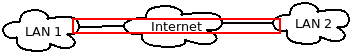
\includegraphics[width=0.9\linewidth]{vpn-site_to_site.png}
	\caption{Site to Site VPN}
	\label{fig:VPNSiteToSite}
	\end{figure}
\item[host-to-network] is een techniek waarbij een gebruiker over een publiek netwerk (WAN) een veilige verbinding maakt met een netwerk alsof hij lokaal op dat netwerk aangesloten is. Zie \ref{fig:VPNHostToNetwork}
	\begin{figure}[h]
	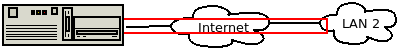
\includegraphics[width=0.9\linewidth]{vpn-host_to_network.png}
	\caption{Host to Network VPN}
	\label{fig:VPNHostToNetwork}
	\end{figure}
\item[host-to-internet] maskeer je IP-adres op Internet door gebruik te maken van een VPN server op Internet waarbij al je verkeer lijkt te komen van deze VPN-server en je dus bijna niet meer te traceren bent. Zie \ref{fig:HostToInternet}
	\begin{figure}[h]
	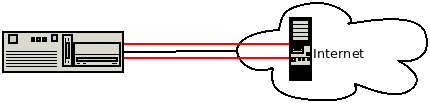
\includegraphics[width=0.9\linewidth]{vpn-host_to_internet.png}
	\caption{Host to Internet VPN}
	\label{fig:VPNHostToInternet}
	\end{figure}
\end{description}

De verschillende soorten VPNs op basis van de techniek:
\begin{description}
\item[Datalink-Layer-VPN] Een VPN die gebruikt maakt van technieken op OSI-layer 2. Voor de erboven gelegen protocolen zou de techniek transparant moeten zijn.
\item[Network-Layer-VPN] Een VPN die gebruikt maakt van technieken op OSI-layer 3. Veelal een vervanging of aanvulling op het IP-protocol.
\item[Transport-Layer-VPN] Een VPN die gebruikt maar van technieken op de transport en applicatie layer om een VPN op te bouwen.
\end{description}


\chapter{Transport-layer}
\section{Implementations}
\subsection{OpenVPN}
\subsection{tinc}
\subsection{SoftEther}
\subsection{FreeLAN}
\subsection{Cisco Adaptive Security Appliance en OpenConnect, AnyConnect}
\subsection{Pulse Secure VPN}

\chapter{Network-layer}
\section{IPsec}
IPsec is een afkorting van Internet Protocol Security. Is een verzameling van protocollen die er gezamenlijk voor zorgen dat data veilig over een IP netwerk gaan. IPsec werkt op OSI-layer 3 en is transparant voor alle bovenliggende lagen zoals TCP en UDP.

De protocollen die IPsec gebruikt zijn:
\begin{description}
\item[IKE] Internet Key Exchange - Een protocol die ervoor zorgt dat de twee end-points van een VPN-tunnel dezelfde keys/certificaten gebruiken om de data te encrypten en decrypten.
\item[ESP] Encapsulating Security Payload - Is een protocol dat voor de encryptie (confidentiality) zorgt en zorgt tevens voor de authenticatie, bescherming tegen replay attacks en interiteitschecks.
\item[AH] Authentication Header - Is een protocol dat er voor zorgt dat als een packet onderweg gewijzigd is (tampering) dat dit gedetecteerd wordt. Door het verzonden packet te signen met het de Authentication Header kan de intergiteit (integrity) worden aangetoond, de AH doet geen encryptie en de gesignde data blijft dus leesbaar als er geen encryptie protocol wordt gebruikt.
\end{description}

IPsec kent twee manieren waarop het gebruikt kan worden:
\begin{description}
\item[Transport Mode] Gebruikt geen encryptie of alleen encryptie voor de (IP) payload. De IP header is dus niet encrypt. Het kan gebruikt worden voor bijvoorbeeld de communicatie tussen een werkstation en een server (host-to-server). Als AH wordt gebruikt dan is de IP header gehashed en kan dus niet meer veranderd worden, ook niet door een NAT-router. Een wijziging zou het totale packet als ongeldig bestempelen (Een mogelijke oplossing is door gebruik te maken van NAT-T \url{https://en.wikipedia.org/wiki/NAT_traversal}).

\item[Tunnel Mode] Het complete IP packet wordt encrypt en opnieuw in een IP packet ingepakt voor verzending over het publieke netwerk. Het wordt vaak gebruikt tussen twee routers/gateways over het Internet om netwerken (site-to-site) aan elkaar te verbinden of om een host aan een netwerk (host-to-network) te verbinden. Tunnel Mode is wat we in het dagelijkse spraakgebruik een VPN noemen.
\end{description}


\section{Implementaties}
\subsection{FreeSWAN, OpenSWAN, StrongSWAN, LibreSWAN}
\subsection{Microsoft}
\section{WireGuard}

\chapter{Datalink-layer}
\section{PPTP}
\section{L2TP}


%%%%%%%%%%%%%%%%%%%%%
%%% Index and End %%%
%%%%%%%%%%%%%%%%%%%%%
%\backmatter
\printindex
\end{document}

%%% Last line %%%
